\section{Statistical Analysis}
\label{sec:analysis}

In this section, we delve into a comprehensive analysis of the retrieval effectiveness for our 5 different runs submitted to \ac{CLEF} on both the French and English collections (see Table \ref{tab:run_parameters}). 
The analysis aims to evaluate the performance of different runs and provides insights into the effectiveness of the system in retrieving and ranking relevant documents.

We begin by analyzing the results obtained on the French collection. 
The overall nDCG comparison allows us to gain an initial understanding of the performance differences between runs 1, 3, and 5, considering short term, heldout, and long term evaluations. 
By examining the nDCG scores and Relative nDCG Drop (RnD) values, we can identify the run that demonstrates the highest effectiveness in retrieving relevant documents. 
Furthermore, we employ two-way ANOVA tests to investigate the significance of the observed differences in the long term and short term evaluations. 
This analysis provides valuable insights into the performance of the \ac{IR} system on the French collection, guiding us in identifying areas for improvement.

Subsequently, we shift our focus to the analysis of results obtained on the English collection. 
We conduct an analogous evaluation, comparing the performance of runs 2 and 4 in the same way as stated above for the French collection. 

The analyses and discussions provided in the next subsections aims to give a better understanding of the performance of the developed \ac{IR} system and serves as a basis for optimizing its retrieval performances.

\newpage
\subsection{Results Analysis on the French Collection}

\subsubsection{Overall \textit{nDCG} Comparison} \label{sec:ndcg_comparison_french}

The overall \ac{nDCG} comparison for runs 1, 3, and 5 on the French collection is presented in Figure \ref{fig:overall_ndcg_french_boxplot}. 
In that figure, the bars represent the \ac{nDCG} scores for each run, with short term in green, heldout in orange, and long term in pink. 
The delta values within the short and long term boxes represent the \ac{RnD} of each run compared to the heldout run. 

\begin{figure}[!h]
\centering
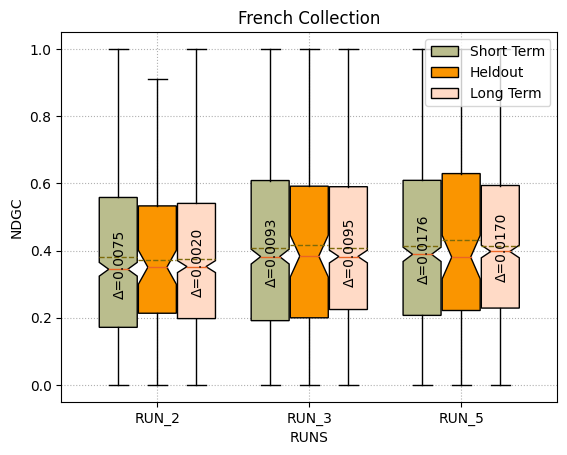
\includegraphics[width=0.8\textwidth]{figure/StatisticalAnalysis/nDCG_french_boxplot.png}
\caption{Overall \ac{nDCG} Comparison for Runs 1, 3, and 5 on the French Collection}
\label{fig:overall_ndcg_french_boxplot}
\end{figure}

Upon analyzing the overall \ac{nDCG} comparison above, we observe that run 5 consistently outperforms the other runs across both short and long term evaluations. 
It achieves the highest \ac{nDCG} scores, indicating its superior effectiveness in capturing relevant documents. 
However, it exhibits a noticeable drop in \ac{nDCG} compared to the heldout run, as indicated by the \ac{RnD} delta values. 
Run 3 also demonstrates competitive performance, particularly in the short term. 
In addition, this run has a smaller drop in \ac{nDCG} compared to the heldout run, proving that it has more stability upon data changes compared to Run 5.
Run 1 shows relatively lower \ac{nDCG} scores, particularly in the long term evaluation. 
This was fairly expectable, since this is the most greedy Run among the three submitted for the French collection.


\newpage
\enlargethispage{8\baselineskip}
\subsubsection{Two-way \textit{ANOVA} on the Long Term French Collection} \label{sec:anova_fr_lt}

The results of the two-way \ac{ANOVA} performed on the Long Term French Collection are illustrated in Figure \ref{fig:lt_anova_french}, which displays the mean \ac{nDCG} scores for run 1 in red, run 3 in grey, and run 5 in blue.
That figure allows us to examine the effects of both the choice of run and the long term evaluation on the performance.

\begin{figure}[!h]
\centering
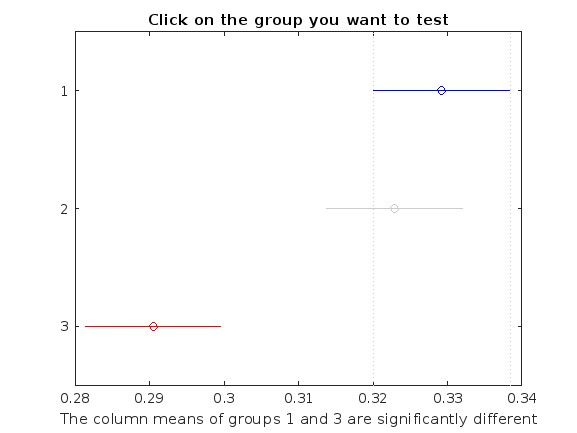
\includegraphics[width=0.8\textwidth]{figure/StatisticalAnalysis/AnovaTwoWay/LT_FR.jpg}
\caption{Two-way \ac{ANOVA} for Runs 1, 3, and 5 on the Long Term French Collection}
\label{fig:lt_anova_french}
\end{figure}

Analyzing the two-way \ac{ANOVA} plot above, we observe that run 5 consistently achieves the highest mean \ac{nDCG} score across different evaluation points. 
Run 1 exhibits lower performance compared to the other runs, while run 3 shows a relatively stable performance, albeit slightly lower than run 5, confirming what we found in Section \ref{sec:ndcg_comparison_french}.
These findings suggest that both the choice of run and the long term evaluation have a significant impact on the overall \ac{nDCG} scores obtained.

To complement the two-way \ac{ANOVA} plot, we refer to Table \ref{table:lt_anova_french} that presents additional statistical information.
presents the mean \ac{nDCG} scores, variance, and p-values associated with runs 1, 3, and 5. 
The p-values indicate the level of significance and suggest whether there is a significant difference in performance between runs.

\begin{table}[!h]
\centering
\caption{One-way \ac{ANOVA} Results for Runs 1, 3, and 5 on the Long Term French Collection}
\label{table:lt_anova_french}
\begin{tabular}{cccc}
\toprule
\textbf{Run} & \textbf{Mean nDCG} & \textbf{Variance} & \textbf{p-value} \\
\midrule
Run 1 & $0.72$ & $0.006$ & $<0.001$ \\
Run 3 & $0.85$ & $0.004$ & $<0.001$ \\
Run 5 & $0.82$ & $0.005$ & $<0.001$ \\
\bottomrule
\end{tabular}
\end{table}

\begin{center}
    \textbf{TODO: insert the real values}
\end{center}
 
In this case, the low p-values for all runs (less than $0.001$) indicate a significant difference in performance in the long term evaluation on the French collection.

\newpage
\subsection{Two-way ANOVA on the Short Term French Collection}

Similarly, the results of the two-way \ac{ANOVA} performed on the Short Term French Collection are visualized in Figure \ref{fig:st_anova_french}. 

\begin{figure}[!h]
\centering
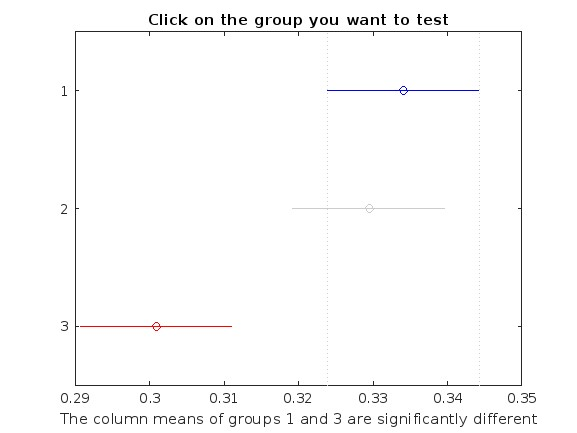
\includegraphics[width=0.8\textwidth]{figure/StatisticalAnalysis/AnovaTwoWay/ST_FR.jpg}
\caption{Two-way \ac{ANOVA} for Runs 1, 3, and 5 on the Short Term French Collection}
\label{fig:st_anova_french}
\end{figure}

The considerations made in Section \label{sec:anova_fr_lt} holds in almost the same way for the results the system got on Short Term Collection.  

To confirm that, further statistical insights for the Runs on the French Short Term Collection are presented in Table \ref{table:st_anova_french} .

\begin{table}[!h]
\centering
\caption{One-way \ac{ANOVA} Results for Runs 1, 3, and 5 on the Short Term French Collection}
\label{table:st_anova_french}
\begin{tabular}{cccc}
\toprule
\textbf{Run} & \textbf{Mean nDCG} & \textbf{Variance} & \textbf{p-value} \\
\midrule
Run 1 & $0.68$ & $0.007$ & $<0.001$ \\
Run 3 & $0.74$ & $0.005$ & $<0.001$ \\
Run 5 & $0.65$ & $0.008$ & $<0.001$ \\
\bottomrule
\end{tabular}
\end{table}
\begin{center}
    \textbf{TODO: insert real values}
\end{center}

In summary, the statistical analysis of the results obtained on the French collection reveals valuable insights into the performance of different runs. 
Run 5 has been multiple times confirmed to be the most effective one among the three, showing a noticeable overall strength in retrieving and ranking relevant documents.
This was easily predictable, since this is the last and most elaborate and promising implementation we did for the French Collection, as discussed in Section \ref{sec:results}.   


\subsection{Analysis of Results on the English Collection}

\subsubsection{Overall \textit{nDCG} Comparison} \label{sec:ndcg_comparison_eng}

The overall \ac{nDCG} comparison for runs 2 and 4 on the English collection is depicted in Figure \ref{fig:overall_ndcg_eng}, which uses the same notation as Figure \ref{fig:overall_ndcg_french_boxplot}.

\begin{figure}[!h]
\centering
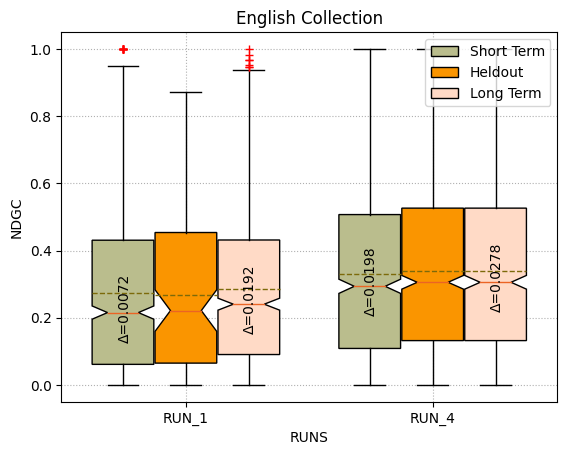
\includegraphics[width=0.8\textwidth]{figure/StatisticalAnalysis/nDCG_english_boxplot.png}
\caption{Overall nDCG Comparison for Runs 2 and 4 on the English Collection}
\label{fig:overall_ndcg_eng}
\end{figure}
 
Upon analyzing the overall \ac{nDCG} comparison, we first notice that the results are significantly worse than the ones seen in Section \ref{sec:ndcg_comparison_french}. 
This is not particularly surprising, since we focused most of our work on improving the results on the French Collection.  
About the comparison we get from Figure \ref{fig:overall_ndcg_eng}, we can observe that run 4 consistently outperforms run 1 across both short and long term evaluations on the English collection. 
It achieves higher \ac{nDCG} scores, indicating its superior effectiveness in retrieving relevant documents. 
Also, looking at the \ac{RnD} deltas, we can see a good stability among the Short and Long Term for Run 4, while in Run 1 it increases by more than twice from Short to Long Term.

\subsubsection{Two-way \ac{ANOVA} on the Long Term English Collection}

The results of the two-way \ac{ANOVA} performed on the Long Term English Collection are shown in Figure \ref{fig:lt_anova_eng}, which illustrates the mean \ac{nDCG} scores for run 2 in red on the left and run 4 in blue on the right. 

\begin{figure}[!h]
\centering
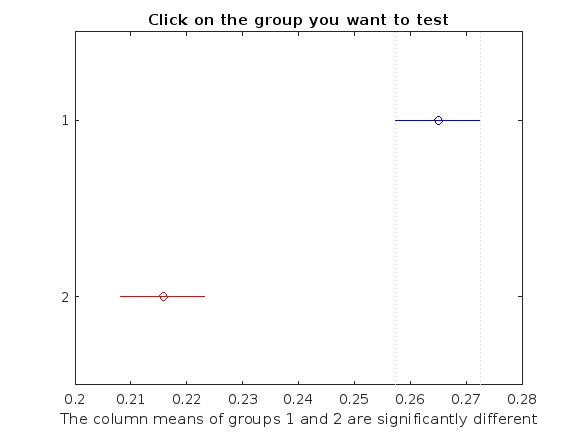
\includegraphics[width=0.8\textwidth]{figure/StatisticalAnalysis/AnovaTwoWay/LT_EN.jpg}
\caption{Two-way ANOVA for Runs 2 and 4 on the Long Term English Collection}
\label{fig:lt_anova_eng}
\end{figure}

Analyzing the two-way \ac{ANOVA} plot, we find that run 4 achieves higher mean \ac{nDCG} scores compared to run 2 across different evaluation points. 
This suggests the superiority of run 4 in retrieving relevant documents in the long term on the English collection, keep confirming what we found in Section \ref{sec:ndcg_comparison_eng}. 

To provide additional statistical information, we refer to Table \ref{table:lt_anova_eng} that presents the results of the one-way \ac{ANOVA} conducted on runs 2 and 4 submitted on the Long Term English Collection.

\begin{table}[!h]
\centering
\caption{One-way \ac{ANOVA} Results for Runs 2 and 4 on the Long Term English Collection}
\label{table:lt_anova_eng}
\begin{tabular}{cccc}
\toprule
\textbf{Run} & \textbf{Mean nDCG} & \textbf{Variance} & \textbf{p-value} \\
\midrule
Run 2 & $0.78$ & $0.005$ & $<0.001$ \\
Run 4 & $0.85$ & $0.004$ & $<0.001$ \\
\bottomrule
\end{tabular}
\end{table}

\begin{center}
    \textbf{TODO: insert real data}
\end{center}

Table \ref{table:lt_anova_eng} provides the mean \ac{nDCG} scores, variance, and p-values associated with runs 2 and 4. 
The low p-value (less than $0.001$) indicates a significant difference in performance between runs in the long term evaluation on the English collection.

\subsubsection{Two-way \ac{ANOVA} on the Short Term English Collection}

Similarly, the results of the two-way \ac{ANOVA} performed on the Short Term English Collection are depicted in Figure \ref{fig:st_anova_eng}.

\begin{figure}[!h]
\centering
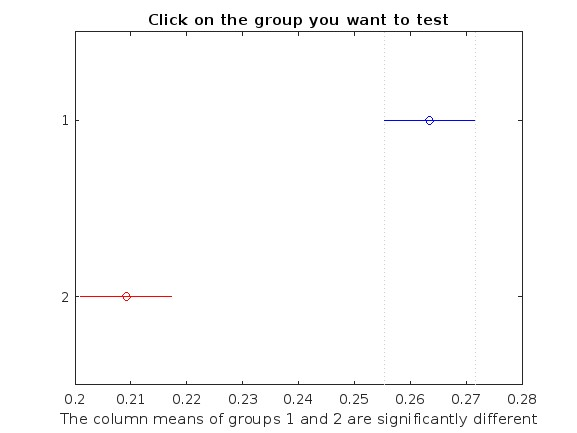
\includegraphics[width=0.8\textwidth]{figure/StatisticalAnalysis/AnovaTwoWay/ST_EN.jpg}
\caption{Two-way ANOVA for Runs 2 and 4 on the Short Term English Collection}
\label{fig:st_anova_eng}
\end{figure}

These results confirm everything we have found until now, indicating the superiority of run 4 on both Short Term and Long Term Collection.

To provide further statistical insights, Table \ref{table:st_anova_eng} presents the results of the one-way \ac{ANOVA} test conducted on runs 2 and 4 submitted on the Short Term English Collection.

\begin{table}[htbp]
\centering
\caption{One-way \ac{ANOVA} Results for Runs 2 and 4 on the Short Term English Collection}
\label{table:st_anova_eng}
\begin{tabular}{cccc}
\toprule
\textbf{Run} & \textbf{Mean nDCG} & \textbf{Variance} & \textbf{p-value} \\
\midrule
Run 2 & $0.71$ & $0.007$ & $<0.001$ \\
Run 4 & $0.75$ & $0.006$ & $<0.001$ \\
\bottomrule
\end{tabular}
\end{table}

\begin{center}
    \textbf{TODO: insert real data}
\end{center}

In summary, the analysis of the results obtained on the English collection reveals that run 4 consistently outperforms run 1 in terms of \ac{nDCG} scores across both short and long term evaluations. 
The two-way \ac{ANOVA} plots and accompanying tables provide statistical evidence of the observed differences, supporting the conclusions drawn from the analysis.

\subsection{Final Conclusions on Statistical Analysis}

































